% Author: Izaak Neutelings (April 2022)
% Description: MET in the CMS detector
% CMS ECAL granularity: https://cds.cern.ch/record/349375/files/ECAL_TDR.pdf
\documentclass[border=3pt,tikz]{standalone}
\usepackage{amsmath}
\tikzset{>=latex} % set default arrow head as latex

\tikzstyle{calo}=[draw=blue!60!green!50!black,fill=blue!60!green!90!black!70,
                  line width=0.6,rounded corners=0.2]
\tikzstyle{ecal}=[calo,draw=red!90!green!60!black,fill=red!85!green!90!black!80]
\tikzstyle{MET}=[->,red,line width=1.2,dashed]
\newcommand*{\myvec}[1]{\vec{\mkern0mu#1}} % correct misalignment in \vec
\newcommand{\ptmiss}{\myvec{p}_\mathrm{T}^\mathrm{\,miss}}

\begin{document}


% (CMS) EVENT DISPLAY with CALO DEPOSITS, MUON & MET
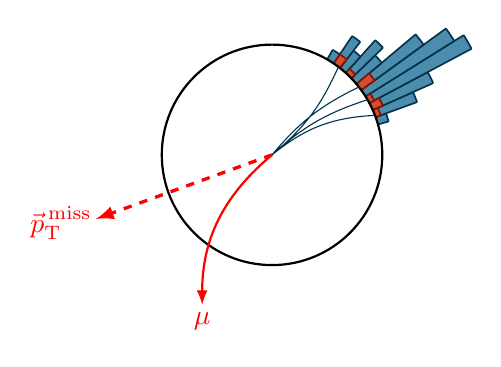
\begin{tikzpicture}[scale=0.7,rotate=0]
  \def\R{2} % tracker outer radius
  \def\dang{4} % angular granularity of calo deposits, CMS: 0.0175*180/pi = 1
  
  %% HELP LINE GRID
  %\draw[black!20,opacity=0.2,very thin]
  %  \foreach \r in {0.2,0.4,...,4.4}{(0,0) circle(\r)}
  %  \foreach \a in {0,10,...,350}{(0,0) -- (\a:4.4)};
  %\draw[black!40,opacity=0.2,thin]
  %  \foreach \r in {1,...,4}{(0,0) circle(\r)}
  %  \foreach \a in {0,30,...,330}{(0,0) -- (\a:4.4)};
  
  % HCAL DEPOSITS
  \foreach \dr [count=\i,
                evaluate={\r=\R+\dr; \anga=12+\dang*\i; \angb=\anga+\dang;}
               ] in {0.2,0.8,1.2,2.1,1.9,1.4,0.6,0.8,0.4,0.6,0.2}{
    \draw[calo] (0,0) -- (\anga:\r) arc(\anga:\angb:\r) -- cycle;
    %\draw[calo]
    %  (\anga:\R) -- (\anga:\r) arc(\anga:\angb:\r)
    %  -- (\angb:\R) arc(\angb:\anga:\R) -- cycle;
  }
  
  % ECAL DEPOSITS
  \foreach \dr [count=\i,
                evaluate={\nz=\dr>0; \r=\R+\dr; \anga=16+\dang*\i; \angb=\anga+\dang;}
               ] in {0.1,0.2,0.1,0.0,0.3,0.0,0.1,0.0,0.2}{
    \ifnum \nz>0
      \draw[ecal] (0,0) -- (\anga:\r) arc(\anga:\angb:\r) -- cycle;
    \fi
  }
  
  % INNER DETECTOR
  \draw[thick,fill=white] (0,0) circle(\R); % fill to hide calo deposits inside
  
  % CHARGED TRACKS
  \draw[blue!60!green!50!black,thin,fill=none]
    (0,0) to[bend left=18] (21:\R)
    (0,0) to[bend left=12] (30:\R)
    (0,0) to[bend left=12] (38:\R)
    (0,0) to[bend right=13] (53:\R);
  
  % MUON TRACK
  \draw[->,thick,red] (0,0) to[out=-140,in=90] (-115:1.5*\R)
    node[below=-1] {$\mu$};
  
  % MET
  \draw[MET] (0,0) -- (-160:1.7*\R)
    node[anchor=6,inner sep=1] {$\ptmiss$}; % MET
  
\end{tikzpicture}


% (CMS) EVENT DISPLAY with CALO DEPOSITS & MET
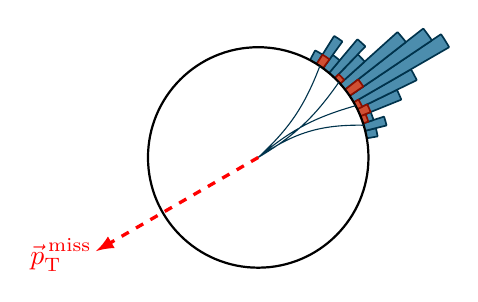
\begin{tikzpicture}[scale=0.7,rotate=0]
  \def\R{2} % tracker outer radius
  \def\dang{4} % angular granularity of calo deposits, CMS: 0.0175*180/pi = 1
  
  % HCAL DEPOSITS
  \foreach \dr [count=\i,
                evaluate={\r=\R+\dr; \anga=6+\dang*\i; \angb=\anga+\dang;}
               ] in {0.2,0.4,0.2,0.8,1.2,2.0,1.8,1.4,0.6,0.8,0.3,0.6,0.2}{
    \draw[calo] (0,0) -- (\anga:\r) arc(\anga:\angb:\r) -- cycle;
    %\draw[calo]
    %  (\anga:\R) -- (\anga:\r) arc(\anga:\angb:\r)
    %  -- (\angb:\R) arc(\angb:\anga:\R) -- cycle;
  }
  
  % ECAL DEPOSITS
  \foreach \dr [count=\i,
                evaluate={\nz=\dr>0; \r=\R+\dr; \anga=14+\dang*\i; \angb=\anga+\dang;}
               ] in {0.1,0.2,0.1,0.0,0.3,0.0,0.1,0.0,0.0,0.2}{
    \ifnum \nz>0
      \draw[ecal] (0,0) -- (\anga:\r) arc(\anga:\angb:\r) -- cycle;
    \fi
  }
  
  % INNER DETECTOR
  \draw[thick,fill=white] (0,0) circle(\R); % fill to hide calo deposits inside
  
  % CHARGED TRACKS
  \draw[blue!60!green!50!black,thin,fill=none]
    (0,0) to[bend left=18] (17:\R)
    (0,0) to[bend left=12] (28:\R)
    (0,0) to[bend right=12] (43:\R)
    (0,0) to[bend right=13] (56:\R);
  
  % MET
  \draw[MET] (0,0) -- (-150:1.7*\R)
    node[anchor=6,inner sep=1] {$\ptmiss$}; % MET
  
\end{tikzpicture}


\end{document}